\documentclass[12pt]{article}

\usepackage{mathtools}
\usepackage{bm}
\usepackage{dsfont}
\usepackage{comment}
\usepackage{amssymb}
\usepackage{amsmath}
\usepackage{dsfont}
\usepackage{comment}
\usepackage[nomarkers,figuresonly]{endfloat}
\usepackage{amsfonts}

\usepackage{multirow}
\usepackage{graphicx}
\usepackage{caption}
\usepackage{subcaption}
\usepackage{float}
\usepackage[section]{placeins}
\usepackage[font=normalsize,labelfont=bf]{caption}
\captionsetup[table]{font=footnotesize,labelfont={sf}}

\usepackage{booktabs, siunitx}
\usepackage{array}
\usepackage{accents}
\usepackage{setspace}
\usepackage[round]{natbib}
\usepackage[titletoc]{appendix}


\usepackage{longtable}
\usepackage{totcount}
\usepackage{alphalph}
\usepackage{tabularx}
\usepackage{rotating}

\usepackage{hyperref} 
\usepackage{fullpage} 
\usepackage{tikz}
\usepackage{pgfplots}
\usepackage{pgfplotstable}
\usetikzlibrary{shapes, arrows.meta, positioning}
\usetikzlibrary{arrows.meta,
                chains,
                positioning,
                shapes.geometric,
                decorations.pathreplacing
                }

\begin{document}
	
\tikzset{%
every neuron/.style={
circle,
draw,
minimum size=1cm
},
neuron missing/.style={
draw=none,
scale=4,
text height=0.333cm,
execute at begin node=\color{black}$\vdots$
},
}

\begin{tikzpicture}[x=1.5cm, y=1.5cm, >=stealth]

\foreach \m [count=\y] in {1,2,3,missing,4}
\node [every neuron/.try, neuron \m/.try] (input-\m) at (0,2.5-\y) {};

\foreach \m [count=\y] in {1,missing,2}
\node [every neuron/.try, neuron \m/.try ] (hidden-\m) at (2,2-\y*1.25) {};

\node[every neuron] (outp) at (4, -.5) {};

\draw[->] (outp) -- ++(1,0) node [above, midway] {$O$};

\foreach \l [count=\i] in {1,2,3,n}
\draw [<-] (input-\i) -- ++(-1,0)
node [above, midway] {$I_\l$};

\foreach \l [count=\i] in {1,n}
\node [above] at (hidden-\i.north) {$H_\l$};

\foreach \i in {1,...,4}
\foreach \j in {1,...,2}
\draw [->] (input-\i) -- (hidden-\j);

\foreach \i in {1,...,2}
\draw [->] (hidden-\i) -- (outp);

\foreach \l [count=\x from 0] in {Input, Hidden, Output}
\node [align=center, above] at (\x*2,2) {\l \\ layer};

\end{tikzpicture}
\newpage 

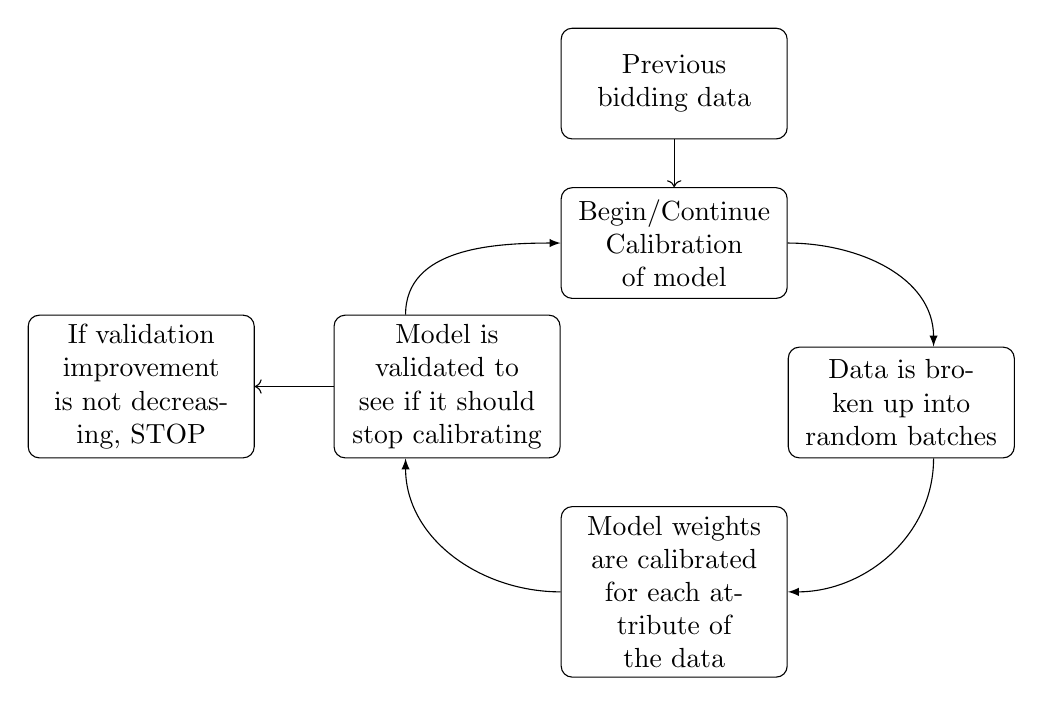
\begin{tikzpicture}[
	node distance=4ex and 0em,
	block/.style={rectangle, draw, fill=white!20, 
		text width=7.5em, text centered, rounded corners, minimum height=4em},
	line/.style={draw, -latex},
	]
	
	\node [block] (0) {Previous bidding data};
	\node [block, below= of 0] (1) {Begin/Continue Calibration of model};
	\node [block, below right= of 1] (2) {Data is broken up into random batches};
	\node [block, below left= of 2] (3) {Model weights are calibrated for each attribute of the data};
	\node [block, above left= of 3] (4) {Model is validated to see if it should stop calibrating};
	\draw [->] (0) -- (1) ;
	\node [block, left = 1cm of 4] (break) {If validation improvement is not decreasing, STOP};
	\draw [->] (4) -- (break) ;  
	\path [line] (1.east) to[out=0, in=90] (2.60);
	\path [line] (2.-60) to[out=-90, in=0] (3.east);
	\path [line] (3.west) to[out=180, in=-90] (4.-120);
	\path [line] (4.120) to[out=90, in=180] (1.west);
\end{tikzpicture}
	\newpage 
	
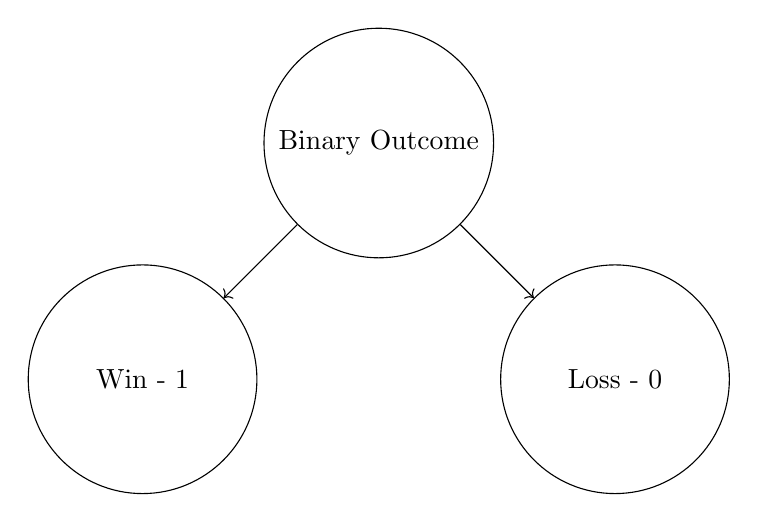
\begin{tikzpicture}[
	node distance=4ex and 0em,
	MyNode/.style={circle, draw, fill=white!20, 
		text width=7.5em, text centered,  minimum height=4em}
	]
	
\node [MyNode] (main) at (0,0) {Binary Outcome}; 
\node [MyNode] (win) at (-3,-3) {Win - 1} ; 
\node [MyNode] (loss) at (3,-3) {Loss - 0} ; 
\draw [->] (main) -- (win);
\draw [->] (main) -- (loss);

\end{tikzpicture}	

\newpage 
\begin{align*}
	\min \ & c^\top x \\ 
	s.t. \ & Ax = b \\
	& x \geq 0. 
\end{align*}

\newpage 
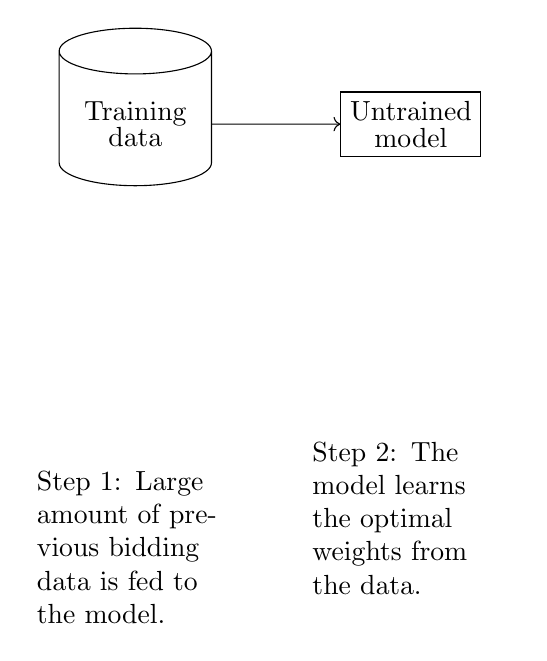
\begin{tikzpicture}[
    node distance = 3.5cm,
    disc/.style = {shape=cylinder, draw, shape aspect=0.3,
                shape border rotate=90,
                text width=17mm, align=center, 
                font=\linespread{0.8}\selectfont,
                minimum height=2cm},
    mdl/.style = {shape=ellipse, aspect=2.2, draw},
    alg/.style = {draw, align=center, font=\linespread{0.8}\selectfont}
                    ]

\node (n1) [disc] {Training\\ data};
\node (n2) [alg, right of=n1]  {Untrained\\ model};
\draw[->] (n1) -- (n2) ;

%\node (n3) [mdl]  {Model};
%\node (n4) [disc] {Test\\ data};
%\node (n3) [mdl]  {Model\\ Validation};
%\node (n3) [mdl]  {Model\\ Shifts};

\node[below=of n1, text width=2.5cm] {Step 1: Large amount of previous bidding data is fed to the model.};
\node[below=of n2, text width = 2.5cm]  {Step 2: The model learns the optimal weights from the data.};


%\path[draw,->] (n1) edge (n2)
 %(n2) edge (n3)
               %(n3) edge (n4)
                    %(otsu.east) -| (right) -- (left) |- (gchannel)
                    %(gchannel) edge (closing)
                    %(closing) edge (NN)
                    %(NN) edge (limit)
                    
    \end{tikzpicture}
    
\newpage 
\begin{align*}
	\min \ & c^\top x \\ 
	s.t. \ & Ax = b \\
	& x \geq 0. 
\end{align*}


\newpage
\begin{tikzpicture}[node distance=3.5cm]
    \draw[shift={(0,0)}, color=black] (0pt,3pt) -- (0pt,-3pt);    
    \draw[shift={(4,0)}, color=red] (0,6pt) -- (0pt, -6pt);
    \draw[shift={(8,0)}, color=green] (0,6pt) -- (0pt, -6pt);
    \draw[shift={(12,0)}, color=black] (0pt,3pt) -- (0pt,-3pt);
    \draw[->, color=green] (8,0) -- (16,0);
    \draw[<-, color=red] (-2,0) -- (4,0);
    \draw[-, color=blue] (4,0)--(8,0);
    \draw (8,-.5) node[below] {100.50}; 
    \node[align=left] at (8,-2) {Winning\\ bid price}; 
    \node[align=left] at (4,2) {Next best\\ bid price};
    \draw (4,.65) node[above] {100.25};
    \draw[decorate, decoration={brace, amplitude=10pt}] (4, 3)--(8,3)
     node[black,midway,yshift=1cm, align=center] {Unrealized gain\\(if winner of auction)};
    \draw[decorate, decoration={brace, amplitude=10pt}] (8,.5)--(16,.5)
     node[black,midway,yshift=1cm, align=center] {Winning\\ bids};  
    \draw[decorate, decoration={brace, amplitude=10pt}] (-2,.5)--(4,.5)
     node[black,midway,yshift=1cm, align=center] {Losing\\ bids};   
    
    % \draw (0,-.5) node[below] {$\ldots$};
    % \draw (2,-.5) node[below] {100.00}; 
    % \draw (6,-.5) node[below] {101.00};
    
    % \draw (8,-.5) node[below] {$\ldots$};
\end{tikzpicture}

\newpage 


\begin{tikzpicture}[domain=0:8]
  \draw[very thin,color=gray, step=2cm] (-0.2,-2.1) grid (7.9,7.9);
  \draw[->] (-0.2,0) -- (8.2,0) node[right] {Actual win rate};
  \draw[->] (0,-2.2) -- (0,8.2) node[above] {Estimated win rate};
  \node[color=black] at (2.0, 2.3) {\Large \textbullet};
  \node[color=black] at (4.0, 3.9) {\Large \textbullet};
  \node[color=black] at (6.0, 4.5) {\Large \textbullet};
  \node[color=red] at (2.0, 2.9) {\Large \textbullet};
  \node[color=red] at (4.0, 3.2) {\Large \textbullet};
  \node[color=red] at (6.0, 2.9) {\Large \textbullet};
  
\draw[decorate, decoration={brace, mirror, amplitude=10pt}] (6,2.9)--(6,4.5)
     node[black,midway,xshift=1cm, align=right] {Gap};   

\end{tikzpicture}

\begin{tikzpicture}[domain=0:8]
  \draw[very thin,color=gray, step=2cm] (-0.2,-2.1) grid (7.9,7.9);
  \draw[->] (-0.2,0) -- (8.2,0) node[right] {Actual win rate};
  \draw[->] (0,-2.2) -- (0,8.2) node[above] {Estimated win rate};
  \node[color=black] at (2.0, 2.3) {\Large \textbullet};
  \node[color=black] at (4.0, 3.9) {\Large \textbullet};
  \node[color=black] at (6.0, 4.5) {\Large \textbullet};
  \node[color=red] at (2.0, 2.5) {\Large \textbullet};
  \node[color=red] at (4.0, 3.7) {\Large \textbullet};
  \node[color=red] at (6.0, 4.7) {\Large \textbullet};
  
\draw[decorate, decoration={brace, mirror, amplitude=10pt}] (6,2.9)--(6,4.5)
     node[black,midway,xshift=1cm, align=right] {Gap};   

\end{tikzpicture}

\end{document}